%You can leave alone everything before Line 79.
\documentclass{article}
\usepackage{url,amsfonts, amsmath, amssymb, amsthm,color, enumerate, verbatim}
% Page layout
\setlength{\textheight}{8.75in}
\setlength{\columnsep}{2.0pc}
\setlength{\textwidth}{6.5in}
\setlength{\topmargin}{0in}
\setlength{\headheight}{0.0in}
\setlength{\headsep}{0.0in}
\setlength{\oddsidemargin}{0in}
\setlength{\evensidemargin}{0in}
\setlength{\parindent}{1pc}
\newcommand{\shortbar}{\begin{center}\rule{5ex}{0.1pt}\end{center}}
%\renewcommand{\baselinestretch}{1.1}
% Macros for course info
\newcommand{\courseNumber}{ME 552}
\newcommand{\courseTitle}{Mechatronics}
\newcommand{\semester}{Fall 2012}
\newcommand{\xxx}[1]{\textcolor{red}{#1}}
% Theorem-like structures are numbered within SECTION units
\theoremstyle{plain}
\newtheorem{theorem}{Theorem}[section]
\newtheorem{lemma}[theorem]{Lemma}
\newtheorem{corollary}[theorem]{Corollary}
\newtheorem{proposition}[theorem]{Proposition}
\newtheorem{statement}[theorem]{Statement}
\newtheorem{conjecture}[theorem]{Conjecture}
\newtheorem{fact}{Fact}
%definition style
\theoremstyle{definition}
\newtheorem{definition}[theorem]{Definition}
\newtheorem{example}{Example}
\newtheorem{problem}[theorem]{Problem}
\newtheorem{exercise}{Exercise}
\newtheorem{algorithm}{Algorithm}
%remark style
\theoremstyle{remark}
\newtheorem{remark}[theorem]{Remark}
\newtheorem{reduction}[theorem]{Reduction}
%\newtheorem{question}[theorem]{Question}
\newtheorem{question}{Question}
%\newtheorem{claim}[theorem]{Claim}
%
% Proof-making commands and environments
\newcommand{\beginproof}{\medskip\noindent{\bf Proof.~}}
\newcommand{\beginproofof}[1]{\medskip\noindent{\bf Proof of #1.~}}
\newcommand{\finishproof}{\hspace{0.2ex}\rule{1ex}{1ex}}
\def\therefore{\boldsymbol{\text{ }
\leavevmode
\lower0.4ex\hbox{$\cdot$}
\kern-.5em\raise0.7ex\hbox{$\cdot$}
\kern-0.55em\lower0.4ex\hbox{$\cdot$}
\thinspace\text{ }}}

\newenvironment{solution}[1]{\medskip\noindent{\bf Problem #1.~}}{\shortbar}

%====header======
\newcommand{\solutions}[4]{
%\renewcommand{\thetheorem}{{#2}.\arabic{theorem}}
\vspace{-2ex}
\begin{center}
{\small  \courseNumber, \courseTitle
\hfill {\Large \bf {#1} }\\
\semester, University of Michigan, Ann Arbor \hfill
{\em Date: #3}}\\
\vspace{-1ex}
\hrulefill\\
\vspace{4ex}
{\LARGE Lab Assignment #2}\\
\vspace{2ex}
\end{center}
\begin{trivlist}
\item \textsc{Team members:\\} {#4}
\end{trivlist}
\noindent
\shortbar
\vspace{3ex}
}
% math macros
\newcommand{\defeq}{\stackrel{\textrm{def}}{=}}
\newcommand{\Prob}{\textrm{Prob}}
\newcommand{\Lagr}{\mathcal{L}}
\newcommand{\Sens}{\mathcal{S}}
%==
\usepackage{graphicx}
\usepackage{xfrac}
\usepackage{amsmath}
\providecommand{\e}[1]{\ensuremath{\times 10^{#1}}}
\begin{document}
%%%%%%%%%%%%%%%%%%%%%%%%%%%%%%%%%%%%%%%%%%%%%%%%%
%\solutions{Your name}{Problem Set Number}{Date of preparation}{Collaborators}{Prover}{Verifiers}
\solutions{}{6: Inertial Sensors}{\today}{Shiva Ghose, @gshiva\\ John Peterson, @jrpeters\\ Peter Turpel, @pturpel\\ Chan-Rong Lin, @pmelin}
%%%%%%%%%%%%%%%%%%%%%%%%%%%%%%%%%%%%%%%%%%%%%%%%%
%\renewcommand{\theproblem}{\arabic{problem}} 
%%%%%%%%%%%%%%%%%%%%%%%%%%%%%%%%%%%%%%%%%%%%%%%%%
%
% Begin the solution for each problem by
% \begin{solution}{Problem Number} and ends it with \end{solution}
%
% the solution for Problem 
\section*{Teamwork Participation Pledge :: Team 1}

I attest that I have made a fair and equitable contribution to this lab and submitted 
assignment. \\

My signature also indicates that I have followed the University of Michigan Honor Code, 
while working on this lab and assignment.\\

I accept my responsibility to look after all of the equipment assigned to me and my team, 
and that I have read and understood the X50 Lab Rules.\\

\begin{table}[h]
\begin{center}
    \begin{tabular}{|c|c|c|}
        \hline
        \textbf{Name} & \textbf{Email}     & \textbf{ \ \ \ \ \  \ \  \ \ \ \ \  \ \ Signature  \ \ \ \ \  \ \ \ \ \ \ \  \ \ } \\ \hline
        	~& ~& ~\\
	~& ~& ~\\
	Shiva Ghose   & gshiva@umich.edu   & ~                  \\
	~& ~& ~\\
	~& ~& ~\\ \hline 
	~& ~& ~\\
	~& ~& ~\\
        John Peterson & jrpeters@umich.edu & ~                  \\ 
	~& ~& ~\\
	~& ~& ~\\ \hline 
	~& ~& ~\\
	~& ~& ~\\
        Peter Turpel   & pturpel@umich.edu & ~                  \\
	~& ~& ~\\
	~& ~& ~\\ \hline 
	~& ~& ~\\
	~& ~& ~\\
        Chan-Rong Lin   & pmelin@umich.edu & ~                  \\
	~& ~& ~\\
	~& ~& ~\\ \hline 
        \hline
    \end{tabular}
\end{center}
\end{table}

\newpage

\section{Accelerometer Wiring \& Configuration} 

\subsection{Configuration}

Figure \ref{wiring} shows the wiring diagram of the inertial sensor system. The accelerometer is mounted to a breadboard fixed to the the shaft clamp on the encoder such that the plane of the sensor PCB is perpendicular to the plane of axis of rotation of the encoder.  This is necessary because of the limited number of axes available on the rate gyro.  For this assignment we will be making use of the Y and Z axes of the accelerometer and the X axis of the rate gyro (standard and X4.5). We also connected the auto-zero and temperature sensor pins. We are not using the X axis of the accelerometer, the Y axis of the rate gyro (standard and Y4.5), the self-test, or the VRef pins. We used an Arduino Uno as a voltage regulator to provide the encoder with 5V and the IMU with 3.3V.m the Arduino itself was powered from a wall outlet via an AC-to-DC converter.   \\

\begin{figure}[hbt]
\begin{center}
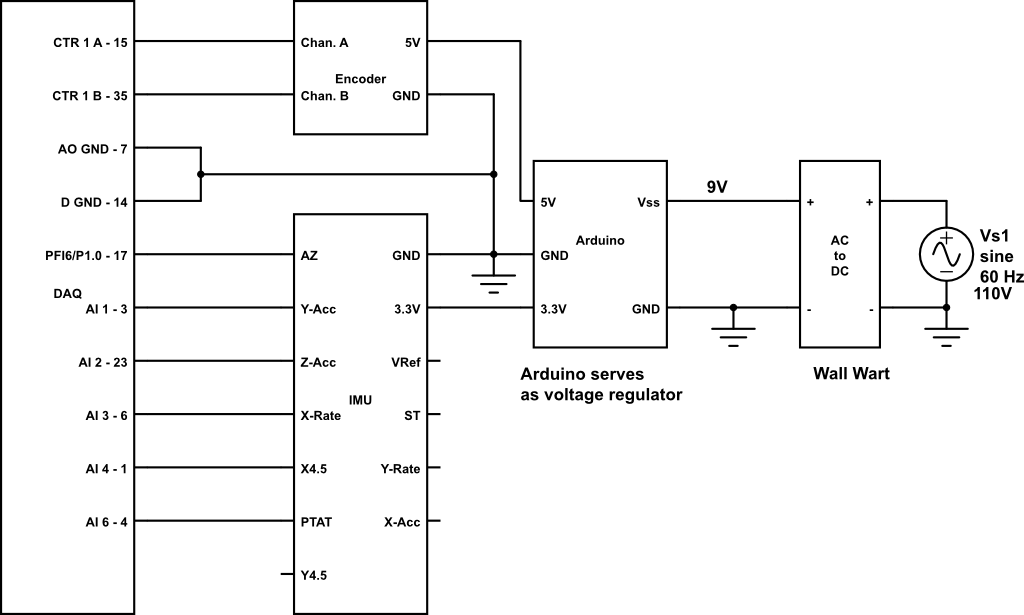
\includegraphics[width = 16cm]{WiringDiagram.png}
\caption{Wiring Connections of Inertial Sensor System.}
\label{wiring}
\end{center}
\end{figure}

\xxx{Confirm that the wiring diagram is correct specifically whether we are using the high or low sensitivity outputs.}

\xxx{Still missing gyro details}

\xxx{We may want a picture of each axis including gyro}

\clearpage

\subsection{Pin Functionality}

\subsubsection{Accelerometer}
Figures \ref{accelPins} and \ref{accelFunc} show the arrangement of the pins on the accelerometer and its functional block diagram, respectively. \\

\begin{figure}[hbt]
\begin{center}
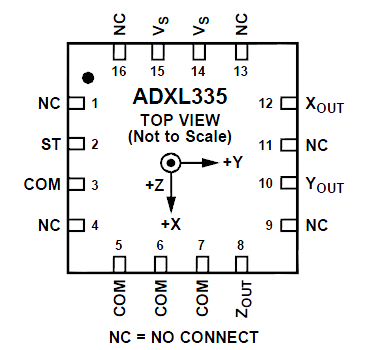
\includegraphics[width = 7cm]{ADXL335Pins.png}
\caption{Pin Configuration of the ADXL335 3-Axis Accelerometer.}
\label{accelPins}
\end{center}
\end{figure}

\begin{figure}[hbt]
\begin{center}
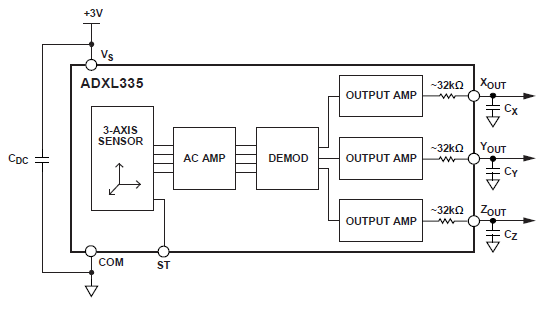
\includegraphics[width = 11cm]{ADXL335Functional.png}
\caption{Functional Diagram of the ADXL335 3-Axis Accelerometer.}
\label{accelFunc}
\end{center}
\end{figure}

\textbf{Pins 1, 4, 9, 11, 13, and 16 - NC}\\
These pins are not connected to the accelerometer's internal circuitry. They are not funcitonal, but they can be connected to ground (the COM pins).\\

\textbf{ Pin 2 - ST}\\
This pin is for the self-test feature of the accelerometer. When the pin is set high by applying the supply voltage an electrostatic force is applied to the accelerometer axes. This results in a known change in the voltage output from each axis. If the change is not seen in the output, this is an indication that there is a problem with the accelerometer. The pin can be connected to ground or left unconnected when not needed. THe PCB provides a connection for this pin, which we did not use.\\

\textbf{Pins 3, 5, 6, and 7 - COM}\\
These pins connect various elements of the accelerometer chip to ground. The PCB provides a connection for ground from the power supply and internally connects this to all of the COM pins. We connected this to the ground terminal of the Arduino.\\

\textbf{Pins 8, 10, and 12 - Z$_{out}$, Y$_{out}$, and X$_{out}$ (respectively)}\\ 
Analog voltage output of the 3 axes of the accelerometer. The accelerometer outputs voltage corresponding to acceleration in the each direction with a range of $\pm$ 3g according to equation \ref{ParamID_EQ1}. The Z axis accelerometer nominally has greater noise density and lower bandwidth compared to the X and Y axes, which are nominally equal. The PCB provides connections for these pins. We connected pins 8 and 10 to the NI breakout board to read with LabView, but did not use pin 12 because that axis (X) was oriented along the shaft's axis of rotation.\\

\textbf{Pins 14 and 15 - V$_s$}\\
Supply voltage for the accelerometer. The accelerometer has a functional supply range of 1.8 V to 3.6 V, with a maximum range of -0.3 V to 3.6 V (based on operation reasonably safe from damage, not functional operation). The accelerometer is ratiometric with typical performance values given based on a V$_s$ of 3 V. Because the output is ratiometric, it is important to use a regulated power supply providing constant voltage. The PCB provides a connection for these pins, which we connected to the 3.3 V terminal of an Arduino Uno.\\ 

\subsubsection{Rate Gyro}
Figures \ref{gyroPins} and \ref{gyroFunc} show the arrangement of the pins on the rate gyro and its functional block diagram, respectively. \\

\begin{figure}[hbt]
\begin{center}
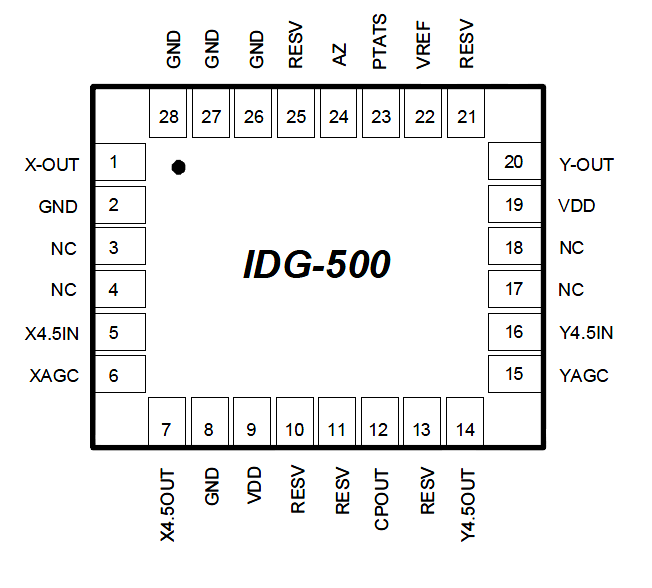
\includegraphics[width = 8cm]{IDG500Pins.png}
\caption{Pin Configuration of the IDG500 Dual-Axis Gyro.}
\label{gyroPins}
\end{center}
\end{figure}

\begin{figure}[hbt]
\begin{center}
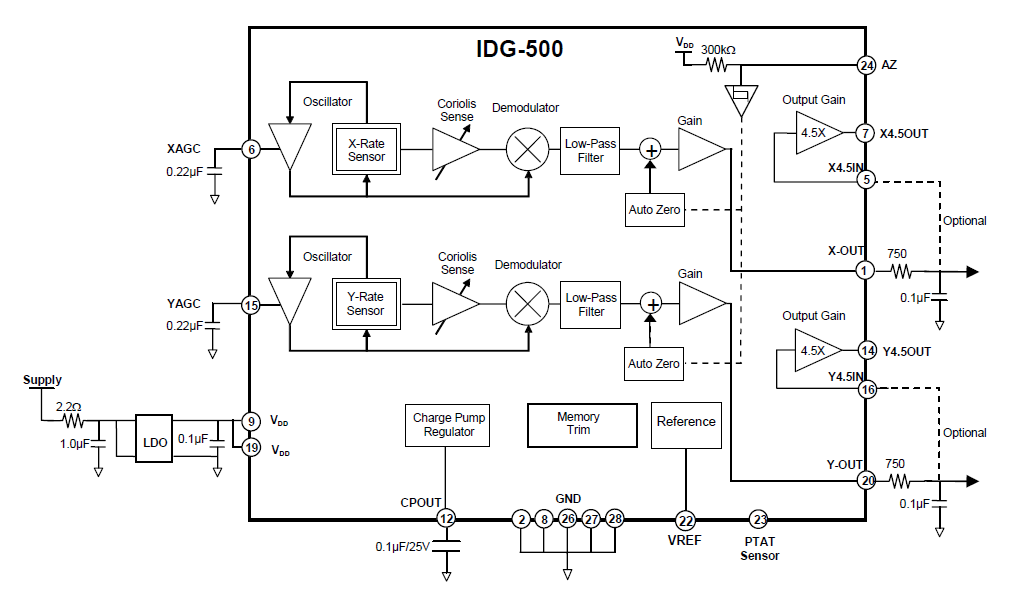
\includegraphics[width = 16cm]{IDG500Functional.png}
\caption{Functional Diagram of the IDG500 Dual-Axis Gyro.}
\label{gyroFunc}
\end{center}
\end{figure}

\textbf{Pins 1 and 20 - X-OUT and Y-OUT (respectively)}\\
Analog output voltage of the X and Y axes of the gyro. The gyro outputs voltage proportional to the angular rate about the X and Y axes according to equation \ref{} \xxx{need equation}. The outputs are not ratiometric and have a nominal full scale range of $\pm$500$^{\circ}$ and sensitivity of 2 $\frac{mV}{^{\circ}/s}$. A low-pass filter is provided internally. The PCB provides connections to these pins. We connected X-OUT to the NI breakout board to read with LabView, but did not connect Y-OUT because our setup did not rotate about that axis.\\

\textbf{Pins 2, 8, 26, 27, and 28 - GND}\\
These pins connect various elements of the gyro chip to ground. The PCB provides a connection for ground from the power supply and internally connects this to all of the GND pins. We connected this to the ground terminal of the Arduino.\\

\textbf{Pins 3, 4, 17, and 18 - NC}\\
These pins are not connected to the gyro's internal circuitry. The data sheet notes that they can be used for PCB trace routing.\\

\textbf{Pins 5 and 16 - X4.5IN and Y4.5IN (respectively)}\\
These pins are inputs to amplifiers which can be connected to X-OUT and Y-OUT to provide higher sensitivity outputs. The connections are optional but are provided internally by the PCB.\\

\textbf{Pins 6 and 15 - XAGC and YAGC (respectively)}\\
These pins provide connections for amplitude control capacitors. 0.22 $\mu$F capacitors are internally used to connect these pins to ground. The capacitors are part of a control loop which controls the amplitude of the internal gains to ensure the sensitivity does not vary with temperature.\\

\textbf{Pins 7 and 14 - X4.5OUT and Y4.5OUT (respectively)}\\
Analog output voltage of the X and Y axes of the gyro. These pins increase the output of X-OUT and Y-OUT by a gain of 4.5 - effectively increasing the sensitivity at the expense of range. The output has a nominal full scale range of $\pm$110$^{\circ}$ and sensitivity of 9.1 $\frac{mV}{^{\circ}/s}$. The PCB provides connections to these pins. We connected X4.5OUT to the NI breakout board to read with LabView, but did not connect Y4.5OUT because our setup did not rotate about that axis.\\

\textbf{Pins 9 and 19 - VDD}\\
Supply voltage for the gyro. The gyro has a functional supply range of 2.7 V to 3.3 V, with a maximum range of -0.3 V to 6.0 V (based on operation reasonably safe from damage, not functional operation). The gyro is not ratiometric and all performance values are based on a VDD of 3 V. The PCB provides a connection for these pins, which we connected to the 3.3 V terminal of an Arduino Uno. A voltage regulator (likely a MIC5205) is included on the PCB betweent the VDD pins and the 3.3 V input connection to ensure the gyro receives 3.0 V. \\ 

\textbf{Pins 10, 11, 13, 21, and 25 - RESV}\\
These pins are reserved and are not connected.\\

\textbf{Pin 12 - CPOUT}\\
Provides an internal connection from ground to a charge pump regulator via a 0.1 $\mu$F capacitor. A charge pump is used for DC/DC regulation and can boost voltages without needing an inductor. \xxx{Might need more explanation here}\\

\textbf{Pin 22 - VREF}\\
A precision reference output which is nominally 1.35 V. Ideally VREF will be a constant 1.35 V and is used with the auto-zero function to reset the zero-rate output to its nominal value of 1.35 V in the event of steady-state drift. The PCB provides a connection to this pin which we did not use.\\

\textbf{Pin23 - PTATS}\\
Provides an output voltage from a temperature sensor within the gyro chip. Output is proportional to temperature with a nominal bias voltage of 1.25 V and a sensitivity of 4 mV/$^{\circ}$C. The PCB provides a connection to this pin which we connected to the NI breakout board and read in LabView (though we did not end up using the data).\\

\textbf{Pin 24 - AZ}\\
This pin is an input to an auto-zero funciton for the X and Y axis gyros. When activated, the auto-zero resets the zero-rate output to be equal to VREF. The auto-zero is typically used when the gyro is not moving to prevent steady-state drift and is supposed to increase the usable range of the high sensitivity outputs (X4.5OUT and Y4.5OUT). The auto-zero is intiated by setting the pin high with a pulse between 2 and 1500 $\mu$s. The PCB provides a connection to this pin with we connected to a digital output of the NI breakout board. In our LabView VI we boolean momentary switch to this output so the user could activate the auto-zero, but this was rarely used.\\ 

\section{Modeling Assumptions}
% there is probably more stuff
\begin{itemize}
\item{Assume that outputs of each axis of the accelerometer and the gyro are independent of one another}
\item{Assume zero bias of each accelerometer axis is stationary} % we may eliminate this assumption if we do online calibration
\item{$g = 9.81 \, \left( \sfrac{m^2}{s}\right) $}
\end{itemize}

\section{Parameter Identification}

\subsection*{Accelerometers}
The basic behavior of an accelerometer, sensitive in the $\hat{u}$ direction is given by equation \ref{ParamID_EQ1} for quasi-static accelerations.  Where $V_{out}$ is the output voltage of the sensor, $V_{bias}$ is the output of the sensor under no acceleration, $V_{supply}$ is the supply voltage to the sensor, and $\Sens$ is a linear approximation of sensor behavior.

\begin{equation}
V_{out} = V_{bias} + \Sens \ddot{u} \quad V_{bias} \approx \frac{V_{supply}}{2}
\label{ParamID_EQ1}
\end{equation}

This response to acceleration can be also be used to measure the acceleration due to gravity along the sensitive axis of an accelerometer allowing the angle between the accelerometer and vertical to be determined.  Let $\theta$ be the measured angle from vertical to the $\hat{y}$ direction of our system.  We can consider two situations, when the sensitive axis is aligned with $\hat{y}$ axis and when it is perpendicular to it.  Let $Y$ and $Z$ denote these situations respectively which correspond to the $\hat{y}$ and $\hat{z}$ axes of our accelerometer.  Then the output voltage of each axis is given as follows:

\begin{equation}
V_{Y} = V_{Ybias} + \Sens_{Y} g \cos(\theta) \quad V_{Z} = V_{Zbias} + \Sens_{Z} g \sin(\theta)
\label{ParamID_EQ2}
\end{equation}

\begin{figure}
\begin{center}
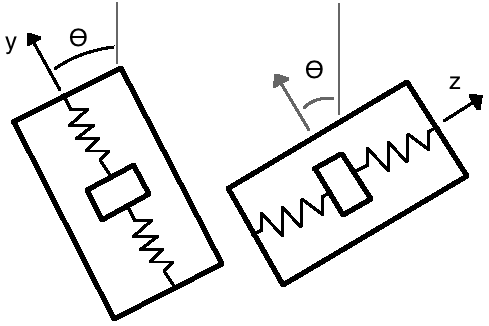
\includegraphics[width = 11cm]{Accelerometer_Cartoon.png}
\caption{Y and Z axis accelerometer}
\label{Accel_cartoon}
\end{center}
\end{figure}

We measured the bias voltage of each axis by fixing the accelerometer such that the axis was perpendicular to the force of gravity and recording the voltage output.  We obtained the bias voltage by averaging these voltages, and we also obtained a measure of noise along each axis by computing the variance of the obtained voltages.  We then conducted a simple experiment where the accelerometer was rotated at slow speeds throughout a complete circle while both axis voltage outputs and encoder angle measurements were recorded.  The equations in \ref{ParamID_EQ2} are linear in the sensitivity values, so we obtained each value through simple least squares regression.  These results are shown in table \ref{ParamID_T} \xxx{not the right table?} \\

% adjust the data sheet values to correspond to if we had a supply voltage of 3.295 Volts, it is ratio metric so it should work
% values as reported by matlab SY = 0.034002931081677, SZ = 0.033903141625302, EY = 2.642681255078259\e{-5}, EZ = 2.774354019095888\e{-4}
\begin{table}
\begin{center}
    \begin{tabular}{|c|c|c|c|c|}
        \hline
        Axis                              & Y Specification & Y   Fit & Z Specification                & Z    Fit                \\ \hline
        $V_{bias} \, (V)$                & 1.5        & 1.617433958  & 1.5         & 1.671451851           \\ 
        $\sigma^2 \, (V^2)$                  & ~      & 1.24553\e{-5}    & ~       & 0.001852504           \\ 
        $\Sens \, \left(\sfrac{V s^2}{m} \right)$                & 0.03058104           & $0.03400293$  & 0.03058104   & $0.03390314$     \\ 
        Fitting Error $(V)$  & - & $2.642681\e{-5}$  & - & $2.774354\e{-4}$ \\
        \hline
    \end{tabular}
\label{ParamID_T}
\caption{Fitting error denotes average error per sample.  Note that the bias voltage and sensitivities quoted in the data sheet are for a supply voltage of 3.0 V, while we are using a supply voltage of 3.295 V}
\end{center}
\end{table}

We see that as reported in the data sheet, the Z-axis is noisier than the Y-axis, but it is to a much greater degree than the data sheet would suggest.  We also see that this extra noise is reflected in the higher fitting errors for the Z-axis data.  

\begin{figure}
\begin{center}
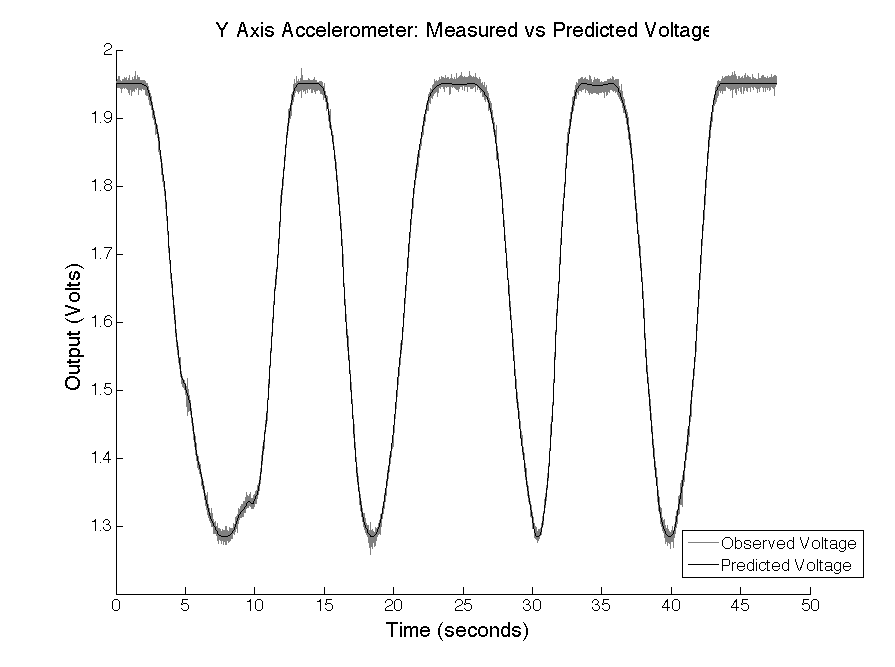
\includegraphics[width = 13cm]{YaxisAccel_Calib.png}
\label{YaccelCalib}
\caption{Expected vs Measured Voltages for the Y axis accelerometer}
\end{center}
\end{figure}

\begin{figure}
\begin{center}
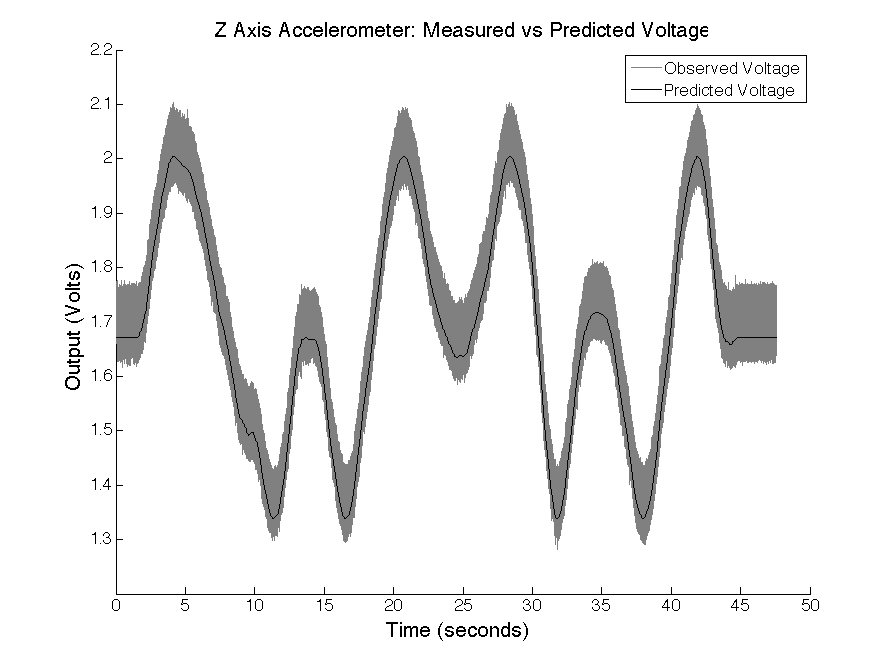
\includegraphics[width = 13cm]{ZaxisAccel_Calib.png}
\label{ZaccelCalib}
\caption{Expected vs Measured Voltages for the Z axis accelerometer}
\end{center}
\end{figure}

\xxx{Compare to the data sheet values still need sigma, they give Noise density, we want sigma, Y = 150 ug/sqrt(Hz) rms, Z = 300}

\subsection*{Rate Gyro}

% note that these calibration results were obtained from the natural frequency with the normal pendulum

A rate gyro gives outputs a voltage proportional to the angular rate about the sensitive axis of the gyro with some offset, the Zero Rate which is not ratiometric.  

$$V_{out} = ZeroRate + \Sens_{Gyro} \dot{\theta} $$

However even of the time period of a few seconds, we encountered several difficulties in trying to apply such a model.  First of all, the rate gyro's response is limited to higher frequencies requiring us to use an oscillating calibration run at the natural frequency of our pendulum sensor set up, of approximately 1.41 Hz.  The data was trimmed to only include the region of the response of a high enough frequency to be within the bandwidth of the sensor.  Secondly, even over this shorter calibration run, the Zero Rate was no constant.  To overcome these difficulties, we fit a slightly more complex model to obtain a good value for the sensitivity.

$$V_{out} = A t + B + \Sens_{Gyro} \dot{\theta} $$

Both $A$ and $B$ vary with time and other variables, such as temperature, so $B$, the zero rate of the gyro is determined on line and A is neglected, so their values for this particular run are irrelevant.  

\xxx{redo at a higher frequency?}
% note that these results were taken at 1.41 Hz, the natural frequency of the normal pendulum
% quoted sensitivity = 1 / 8.635380
\begin{table}
\begin{center}
    \begin{tabular}{|c|c|c|}
        \hline
        ~                                                         & Data Sheet Value & Fit Value \\ \hline
        $\Sens_{Gyro} \, \left( \sfrac{V s}{rad} \right)$ & 0.36             & 0.115803  \\
	$\sigma \, \left( V^2 \right)$ & - & $3.77300 \e{-6}$ \\
	Fitting Error $(rad)$ & - &  $3.35845 \e{-4}$ \\
        \hline
    \end{tabular}
\label{ParamID_TGyro}
\caption{Gyro Sensitivity at 1.41 Hz.}  
\end{center}
\end{table}

\begin{figure}
\begin{center}
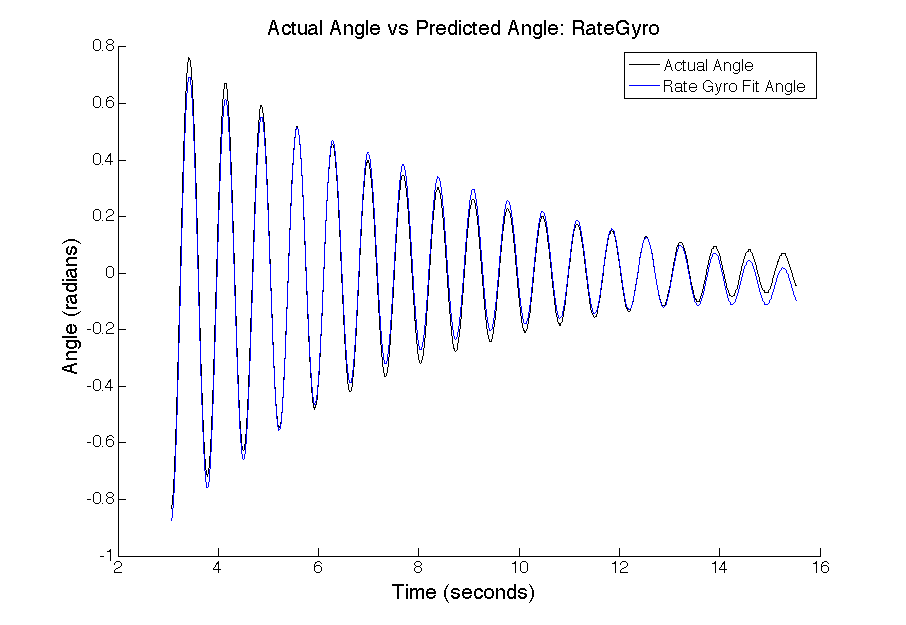
\includegraphics[width = 13cm]{rateGyroCalibResultsS8_636380.png}
\label{gyroCalib}
\caption{Actual Angle vs Fitted Angle from integrating rate gyro output}
\end{center}
\end{figure}

\clearpage
\section{Low Frequency Characterization}

%%%%%%%%%%%%%%%%%%%%%%%%%%%%%%%%%%%%%%%%%%%%%%%%%%%%%%%%%
\subsection{Horizontal Accelerometer}

\subsubsection{Angle Measurement}

Using a single accelerometer in the horizontal configuration is equivalent to just using the Z axis in our configuration.  Where $V_{Z}$ is given as follows: 

$$ V_{Z}(\theta) = V_{Zbias} + \Sens_{Z} g \sin(\theta) $$

$\theta$ can be easily computed by the following expression:

\begin{equation}
\theta = \sin^{-1}\left( \frac{V_{Z} - V_{Zbias}}{\Sens_{Z} g}\right) 
\label{horizontalEQ}
\end{equation}

When using a single accelerometer in the horizontal configuration aliasing occurs for $|\theta| \geq \sfrac{\pi}{2}$.

\xxx{Signal Conditioning?}

\subsubsection{Sensitivity}

The relationship between sensor output voltage and angle is non-linear, but we are able to linearize about a particular operating point, for this experiment, $\theta = 0$, and obtain an estimate of the sensitivity.

$$ V_{Z}(\theta) \approx V_{Zbias} + \Sens_{Z} g \sin(0) + \Sens_{Z} g \cos(0) \left(\theta - 0\right) = V_{Zbias} + \Sens_{Z} g \theta $$

For the horizontal accelerometer, we expect the sensitivity to be $\Sens_{Z} g$. 

\xxx{still need the real results here?}

\subsubsection{Noise}

An estimate for the expected noise in measurement of $\theta$ can be obtained by performing a variance projection through the partial derivative of equation \ref{horizontalEQ}.

$$ \frac{\partial \theta}{\partial V_{Z}} =  \frac{1}{\sqrt{(\Sens_{Z} g)^2 - (V_{Z} - V_{Zbias})^2}}$$

$$ \sigma^2_{\theta} = \frac{\partial \theta}{\partial V_{Z}} \sigma^2_{V_{Z}} \frac{\partial \theta}{\partial V_{Z}} $$

$$ \sigma^2_{\theta} = \frac{\sigma^2_{V_{Z}}}{(\Sens_{Z} g)^2 - (V_{Z} - V_{Zbias})^2}$$

For $\theta \approx 0$ we would expect the noise of our angle measurements to be given by:

$$ \theta \approx 0 \quad \sigma^2_{\theta} \approx \frac{\sigma^2_{V_{Z}}}{(\Sens_{Z} g)^2}$$

% we could plot \sigma^2_theta with respect to theta if we wanted to
\xxx{need to compare to real noise about this point, but our math should be exactly correct}

% comparison to real data here
\begin{table}
\begin{center}
    \begin{tabular}{|c|c|c|}
        \hline
        ~                   & Theoretical  & Actual \\ \hline
        $\sigma^2_{V_{Z}}$    & 0.001852504            & ~      \\ 
        $\sigma^2_{\theta}$ & ~            & ~      \\ 
        $\mu_{V_{Z}}$       & 1.671451851            & ~      \\ 
        $\mu_{\theta}$      & ~            & ~      \\
        \hline
    \end{tabular}
\label{Noise_horizontal_T}
\caption{Comparison of theoretical noise in $\theta$ with measured noise in $\theta$ for the horizontal accelerometer alone. \emph{Note that the theoretical variance of voltage was measured in another trial.}}
\end{center}
\end{table}

%%%%%%%%%%%%%%%%%%%%%%%%%%%%%%%%%%%%%%%%%%%%%%%%%%%%%%%%%
\subsection{Vertical Accelerometer}

\subsubsection{Angle Measurement}

Using a single accelerometer in the vertical configuration is equivalent to using just the Y axis in our configuration.  Where $V_{Y}$ is given as follows:

$$ V_{Y} = V_{Ybias} + \Sens_{Y} g \cos(\theta) $$

Then $\theta$ is given by the following expression:

\begin{equation}
\theta = \cos^{-1}\left( \frac{V_{Y} - V_{Ybias}}{\Sens_{Y} g}\right)
\label{verticalEQ}
\end{equation}

When using a single accelerometer in this configuration aliasing occurs for angles beyond the range $0 \leq \theta \leq \pi$.  This range is much less useful than the range for a single accelerometer in the horizontal configuration because we are unable to read negative angles immediately next to our starting condition, $\theta = 0$. 

\xxx{Signal Conditioning?}

\subsubsection{Sensitivity}

However attempting to linearize about $\theta = 0$ for the accelerometer in the vertical configuration is not nearly as successful.  Yielding a relationship that does not depend on $\theta$ at all.  This result is expected from our earlier assesment of the angle ambiguity between positive values of $\theta$ and negative values.  

$$V_{Y}(\theta) \approx V_{Ybias} + \Sens_{Y} g \cos(0) - \Sens_{Y} g \sin(0) (\theta - 0) = V_{Ybias} + \Sens_{Y} g $$

\xxx{still need the real results here}

\subsubsection{Noise}

We can again use variance projection to estimate the noise in our angle measurements, taking the partial derivative of equation \ref{verticalEQ}.

$$ \frac{\partial \theta}{\partial V_{Y}} = -\frac{1}{\sqrt{(\Sens_{Y} g)^2 - (V_{Y} - V_{Ybias})^2}}$$

$$ \sigma^2_{\theta} = \frac{\partial \theta}{\partial V_{Y}} \sigma^2_{V_{Y}} \frac{\partial \theta}{\partial V_{Y}} $$

$$ \sigma^2_{\theta} = \frac{\sigma^2_{V_{Y}}}{(\Sens_{Y} g)^2 - (V_{Y} - V_{Ybias})^2}$$

As we would expect, this appears identical to the equation for noise of the horizontally mounted accelerometer.  The difference in behavior is simply the voltage around which we linearize.  Substituting the value for $V_{Y}$ about $\theta = 0$  yields absolutely terrible data compared to the horizontal case.

% is this result just a quirk of the linearization?

$$ \theta \approx 0 \quad \sigma^2_{\theta} \approx \frac{\sigma^2_{V_{Y}}}{(\Sens_{Y} g)^2 - (V_{Ybias} + \Sens_{Y} g - V_{Ybias})^2} = \infty$$

% comparison to real data here

\begin{table}
\begin{center}
    \begin{tabular}{|c|c|c|}
        \hline
        ~                   & Theoretical  & Actual \\ \hline
        $\sigma^2_{V_{Y}}$    & 1.24553\e{-5}  & ~      \\ 
	$\sigma^2_{\theta}$ & $\infty$           & ~      \\ 
	$\mu_{V_{Y}}$       & 1.95100270            & ~      \\
        $\mu_{\theta}$      & 0            & ~      \\
        \hline
    \end{tabular}
\label{Noise_vertical_T}
\caption{Comparison of theoretical noise in $\theta$ with measured noise in $\theta$ for the Y axis accelerometer alone. \emph{Note that the theoretical variance of voltage was measured in another trial.}}
\end{center}
\end{table}


%%%%%%%%%%%%%%%%%%%%%%%%%%%%%%%%%%%%%%%%%%%%%%%%%%%%%%%%%
\subsection{Two Accelerometers}

\subsubsection{Angle Measurement}

We can overcome the aliasing issue  presented in the two configuration by using both the horizontal and vertical, the Z and Y axis, simultaneously.  

$$ \cos(\theta) = \frac{V_Y-V_{Ybias}}{\Sens_{Y} g} \quad \sin(\theta) = \frac{V_{Z} - V_{Zbias}}{\Sens_{Z} g} $$

Combining the two equations gives the following:

$$ \tan(\theta) = \frac{\sin(\theta)}{\cos(\theta)} = \left(\frac{V_{Z} - V_{Zbias}}{\Sens_{Z} g}\right) \left( \frac{\Sens_{Y} g}{V_Y-V_{Ybias}} \right) = \frac{\Sens_{Y}}{\Sens_{Z}} \left( \frac{V_{Z} - V_{Zbias}}{V_{Y} - V_{Ybias}} \right)$$

Using the atan2 function avoids the quadrant ambiguities present in the ordinary $\tan^{-1}$ function giving us an expression for $\theta$ valid for all angles.

$$\theta = \text{atan2}\big( \Sens_{Y} \left( V_{Z} - V_{Zbias}\right),  \Sens_{Z} \left( V_{Y} - V_{Ybias}\right) \big)$$

\xxx{Signal Conditioning?}

\subsubsection{Sensitivity}

\subsubsection{Noise}

$$ \theta = \tan^{-1} \left( \frac{\Sens_{Y} \left( V_{Z} - V_{Zbias}\right)}{\Sens_{Z} \left( V_{Y} - V_{Ybias}\right)} \right) = f(V_{Y},V_{Z})$$

Let 

$$ \vec{x} = \left[ V_Y, V_Z \right]^T $$

Then

$$ \theta = f(\vec{x}) \approx J|_{\vec{x}_0} \left( \vec{x} - \vec{x}_{0}\right) \quad J = \left[ \frac{\partial f}{\partial V_{Y}}, \frac{\partial f }{\partial V_Z} \right] $$

$$ \sigma^2_{\theta} = \Sigma_{\theta} = J \Sigma_{\vec{x}} J^T  \quad 
\Sigma_{\vec{x}} = \left[
\begin{matrix}
\sigma^2_{V_{Y}}  & 0 \\
0 & \sigma^2_{V_{Z}} 
\end{matrix} \right]$$

$$ \sigma^2_{\theta} = \left(\frac{\partial f}{\partial V_{Y}}\right)^2 \sigma^2_{V_{Y}} + \left(\frac{\partial f }{\partial V_Z} \right)^2 \sigma^2_{V_{Z}} $$

$$ \frac{\partial f}{\partial V_{Y}} = \frac{\Sens_Z \Sens_Y \left(V_{Z} - V_{Zbias} \right)}{\Sens^2_Y \left(V_Z - V_{Zbias} \right) ^2 + \Sens^2_Z \left( V_Y - V_{Ybias}\right)^2}$$

$$ \frac{\partial f }{\partial V_Z} = \frac{\Sens_Z \Sens_Y \left(V_{Y} - V_{Ybias} \right)}{\Sens^2_Y \left(V_Z - V_{Zbias} \right) ^2 + \Sens^2_Z \left( V_Y - V_{Ybias}\right)^2}$$

For $\theta = 0$ we can simply plug in the nominal voltages earlier to estimate the noise in this angle measurement.

$$ \theta \approx 0 \quad V_{Z}(\theta) \approx V_{Zbias} + \Sens_{Z} g \theta \quad V_{Y}(\theta)  \approx V_{Ybias} + \Sens_{Y} g $$

$$ \frac{\partial f}{\partial V_{Y}} \approx 0  \quad \frac{\partial f }{\partial V_Z} = \frac{1}{\Sens_{Z} g}$$

$$ \sigma^2_{\theta} \approx \left(0\right)^2 \sigma^2_{V_{Y}} + \left(\frac{1}{\Sens_{Z} g} \right)^2 \sigma^2_{V_{Z}} = \left( \frac{\sigma_{V_Z}}{\Sens_{Z} g} \right)^2$$

\xxx{compare to real system}

% comparison to real system

\begin{table}
\begin{center}
    \begin{tabular}{|c|c|c|}
        \hline
        ~                   & Theoretical  & Actual \\ \hline
        $\sigma^2_{V_{Z}}$    & 0.001852504            & ~      \\ 
	$\mu_{V_{Z}}$       & 1.671451851            & ~      \\ 
	$\sigma^2_{V_{Y}}$ & 1.24553\e{-5}		& ~ \\
	$\mu_{V_{Y}}$       & ~            & ~      \\ 
        $\sigma^2_{\theta}$ & ~            & ~      \\ 
        $\mu_{\theta}$      & ~            & ~      \\
        \hline
    \end{tabular}
\label{Noise_dual_T}
\caption{Comparison of expected noise and actual noise for $\theta = 0$}
\end{center}
\end{table}


%%%%%%%%%%%%%%%%%%%%%%%%%%%%%%%%%%%%%%%%%%%%%%%%%%%%%%%%%
\subsection{Rate Gyro}

\subsubsection{Angle Measurement}

\subsubsection{Sensitivity}

\subsubsection{Noise}

\clearpage
\section{Higher Frequency Characterization}

\clearpage
\section{Sensor Fusion}

\clearpage
\end{document}